\section{Familias de distribuciones asociadas al muestreo de la normal}


Sean $X_1, X_2, \dots, X_n$ variables aleatorias i.i.d. $N(\mu, \sigma^2)$ se verifica que:

\begin{enumerate}
    \item Las distribuciones exactas de $\overline{X}$ y $S^2$ son Normal y Gamma respectivamente:

          \[
              \overline{X} \thicksim N\left(\mu,\frac{\sigma^2}{n}\right)
          \]
          \[
              n \frac{S^2}{\sigma^2} \thicksim \gamma\left( \frac{n-1}{2}, \frac{1}{2}\right)
          \]

    \item $\overline{X}$ y $S^2$ son independientes
\end{enumerate}

\subsection{Chi-cuadrado}

Sea $n = 1, 2, 3 \dots$ diremos que una v.a $X$ tiene una distribución Chi-cuadrado con $n$ grados de libertad
cuando su distribución es $\gamma\left(\frac{n}{2}, \frac{1}{2}\right)$ y lo denotaremos

\[
    X \thicksim \chi^2_n
\]

Por tanto es inmediato comprobar que la variabilidad del muestreo sigue una distribución Chi-cuadrado de $n - 1$
grados de libertad

\[
    n\frac{S^2}{\sigma^2} \thicksim \gamma\left(\frac{n - 1}{2}, \frac{1}{2}\right) = \chi^2_{n - 1}
\]

Si $X_1, X_2, \dots, X_n$ son $n$ variables aleatorias i.i.d. con distribución $N(0,1)$, entonces
$Y = X_1^2 + X_2^2 + \dotsi + X_n^2$ es una variable aleatoria con distribución Chi-cuadrado con $n$
grados de libertad

\[
    Y \thicksim \chi^2_n
\]

\newpage

\begin{figure}[h!]
    \begin{center}
        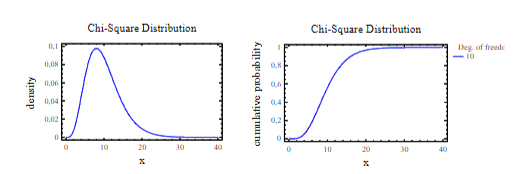
\includegraphics{img/Chi10.png}
    \end{center}
    \caption{Chi-cuadrado con 10 grados de libertad}
\end{figure}

Si $X \thicksim \chi^2_n$ entonces

\[
    EX = n \qquad Var(X) = 2n
\]

La densidad es asimétrica a la derecha y positiva en $(0, \infty)$ \\
Sea $0 < \alpha < 1$ denotamos por $\chi^2_{n,\alpha}$ al $(1-alpha)-cuantil$ de la distribución $\chi^2_n$. Este valor siempre es positivo y está tabulado.

\subsection{F de Fisher-Snedecor}

Sean $n = 1,2,3,\dots$ y $m = 1,2,3,\dots$, y sean $X$ e $Y$ variables aleatorias independientes con distribuciones $\chi^2_n$ y $\chi^2_m$ respectivamente. \\
La distrubición del cociente de las variables se denomina $F$ de Fisher-Snedecor con $n$ y $m$ grados de libertad.

\[
    \frac{\frac{X}{n}}{\frac{Y}{m}} \thicksim F_{n,m}
\]

\begin{figure}[h!]
    \begin{center}
        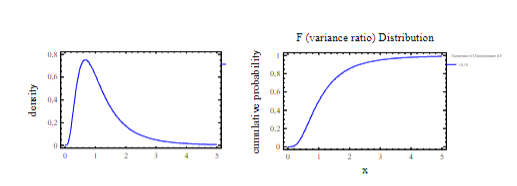
\includegraphics{img/F10.png}
    \end{center}
    \caption{F de Fisher-Snedecor con n = 10, m = 10 grados de libertad}
\end{figure}

Si $X \thicksim F_{n, m}$ entonces

\[
    EX = \frac{m}{m-2} \quad m > 2 \qquad Var(X) = \frac{2m^2(m+n-2)}{n(m-2)^2(m-4)}
\]

Sea $0 < \alpha < 1$ denotamos por $F_{n,m,\alpha}$ al $(1-alpha)-cuantil$ de la distribución $F_{n,m}$. Con esta notación, para usar las tablas de la distribución
debemos tener en cuenta la siguiente propiedad

\[
    F_{n,m,\alpha} = \frac{1}{F_{m,n,1-\alpha}}
\]

\subsection{t de Student}

Sea $n = 1,2,3\dots$ y sean $Z$ y $X$ v.a. independientes con distribuciones $N(0,1)$ y $\chi^2_n$ respectivamente.
La distribución de $\frac{Z}{\sqrt{\frac{X}{n}}}$ se denomina t de Student con $n$ grados de libertad y lo denotaremos

\[
    \frac{Z}{\sqrt{\frac{X}{n}}} \thicksim t_n
\]

\begin{figure}[h!]
    \begin{center}
        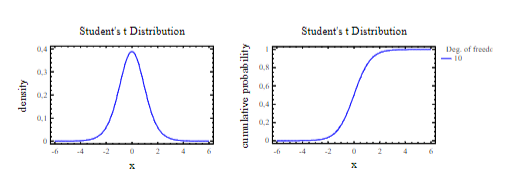
\includegraphics{img/t10.png}
    \end{center}
    \caption{t de Student con 10 grados de libertad}
\end{figure}

Si $X \thicksim t_n$ entonces

\[
    EX = 0 \quad n > 1 \qquad Var(X) = \frac{n}{n-2}
\]

Ademas, la distribución $t_1$ es una $Cauchy(0,1)$ \\

Su densidad es acampanada y simétrica con respecto al origen. Sea $0 < \alpha < 1$ denotamos por $t_{n,\alpha}$ al $(1-alpha)-cuantil$ de la distribución $t_n$. Con esta notación, para usar las tablas de la distribución
debemos tener en cuenta la siguiente propiedad

\[
    t_{n, 1-\alpha} = -t_{n,\alpha}
\]
